% Appendix Template

\chapter{Automated Diagnosis Workflow} \label{Automated Diagnosis Workflow} % Change X to a consecutive letter; for referencing this appendix elsewhere, use \ref{AppendixX}


\section*{AI Powered Medical Scanning}

Chest X-ray and CT scans are the primary screening mechanisms for
diagnosing COVID-19. The limitation to these being the viral 
exposure between the technician and the patient, as assistance 
is required to perfect patient positioning for these scans to 
yield satisfactory results. Therefore, an automated and 
contact-less workflow is the need of the hour.

Modern CT and X-ray systems include cameras to allow 
technicians to remotely monitor the patient. But especially 
since the outbreak of the pandemic, this would not be 
sufficient as technicians would not be able to determine 
scanning parameters such as scan range \cite{SFJ+2020}.

Fortunately, a fully automated scanning workflow is indeed possible 
through AI. Patient pose and shape could be acquired via 
visual sensors such as RGB, Time-of-Flight (TOF) pressure imaging or 
thermal (FIR) cameras. Therefore, optimal scanning parameters could be 
determined \cite{UIH2020, SVK+2017, SVY+2017, SIE2020, LJU+2020, MAR2020, AFA+2020, SIE(2)2020}.

Through this automated scanning workflow, radiation exposure 
can be reduced significantly as well as increasing the overall efficiency of the 
diagnosis procedure \cite{WYX+2020}. Especially during this period of the pandemic, using 
the same workflow would prevent virus exposure between technicians or 
medical practitioners and patients.
\\
\begin{figure}[H]
    \centering
    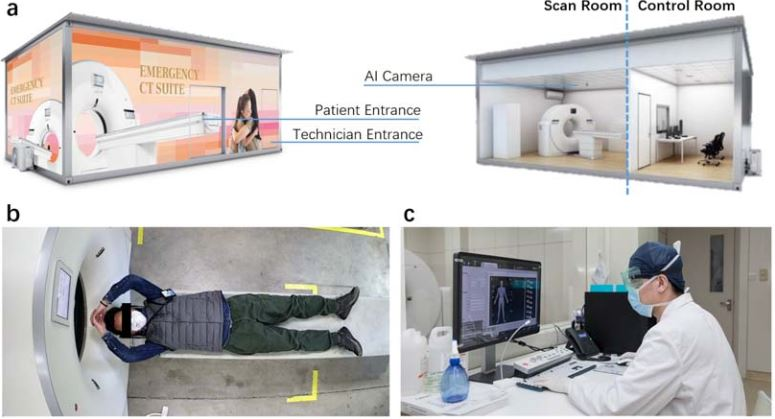
\includegraphics{Images/AutomatedCTScan.JPG}
    \decoRule
    \caption[Mobile CT Platform]{AI-empowered automated image acquisition workflow \cite{SFJ+2020}.}
    \label{fig:Mobile CT Platform}
    \end{figure}

Utilizing this workflow we can procure high-quality X-ray and CT scans suitable for segmentation, but more importantly, we can ensure the safety of both patients and technicians by reducing the radiation and virus exposure respectively. 
% To carry out the automated diagnosis process, segmentation of the 
% lung CT or X-ray scans are a vital pre-requisite in order to identify the regions of interest (ROIs). The former produces 
% high-quality 3D images for detecting COVID-19 whereas the latter involves 
% the ribs being projected onto soft-tissues in 2D. As a result, image segmentation 
% in X-ray scans is more challenging as compared to CT scans. But on the other hand, 
% X-ray scans are more widely accessible in medical facilities all across the world 
% and are usually the first imaging modality used on patients suspected of COVID-19.

% Keeping in mind these limitations, in the next two subsections review the
% image segmentation techniques using deep learning for both CT and X-rays respectively and 
% discuss the results obtained.
